\documentclass[border=10pt]{standalone}
\usepackage{tikz}
\usetikzlibrary{shapes.symbols, arrows.meta}

% Cores personalizadas
\definecolor{corNuvem}{RGB}{189, 212, 231}   % azul claro (preenchimento de A)
\definecolor{bordaNuvem}{RGB}{107, 156, 184} % azul médio (borda de A)
\definecolor{corOval}{RGB}{232, 144, 144}    % rosa (preenchimento de S)
\definecolor{bordaOval}{RGB}{204,  17,  17}  % vermelho (borda de S)
\definecolor{corSeta}{RGB}{ 59, 107, 191}    % azul (seta)

\begin{document}
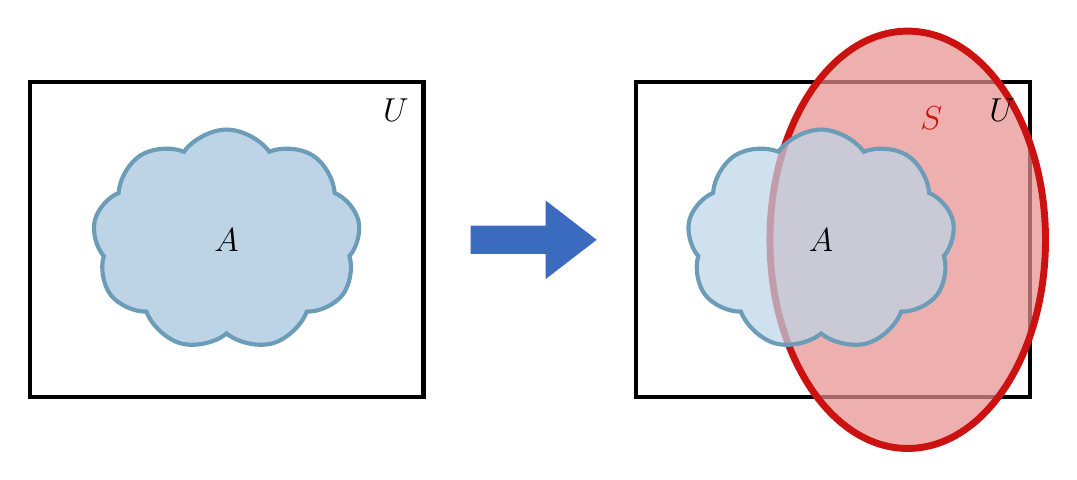
\begin{tikzpicture}

  %% ================================================================
  %%  PAINEL ESQUERDO — apenas o conjunto A dentro do universo U
  %% ================================================================
  \draw[line width=1.5pt] (0,0) rectangle (5,4);

  % Nuvem A
  \node[cloud, cloud puffs=9, cloud puff arc=110,
        minimum width=3.4cm, minimum height=2.8cm,
        fill=corNuvem, draw=bordaNuvem, line width=1.5pt]
        at (2.5, 2) {};
  \node[font=\large\itshape] at (2.5, 2) {$A$};

  % Rótulo U
  \node[font=\large\itshape] at (4.65, 3.65) {$U$};

  %% ================================================================
  %%  SETA
  %% ================================================================
  \fill[corSeta]
    (5.6, 1.82) -- (6.55, 1.82) -- (6.55, 1.50) --
    (7.20, 2.00) --
    (6.55, 2.50) -- (6.55, 2.18) -- (5.6, 2.18) -- cycle;

  %% ================================================================
  %%  PAINEL DIREITO — conjuntos A e S sobrepostos
  %% ================================================================
  \draw[line width=1.5pt] (7.7, 0) rectangle (12.7, 4);

  % Oval S (desenhado primeiro = atrás de A)
  % fill opacity separa a transparência do preenchimento da borda sólida
  \fill[corOval, fill opacity=0.72] (11.15, 2) ellipse (1.75cm and 2.65cm);
  \draw[bordaOval, line width=2.5pt]  (11.15, 2) ellipse (1.75cm and 2.65cm);

  % Nuvem A (na frente; fill opacity cria tom roxo na interseção por mistura)
  \node[cloud, cloud puffs=9, cloud puff arc=110,
        minimum width=3.4cm, minimum height=2.8cm,
        fill=corNuvem, fill opacity=0.72,
        draw=bordaNuvem, line width=1.5pt]
        at (10.05, 2) {};

  % Rótulos do painel direito
  \node[font=\large\itshape]               at (10.05, 2.00) {$A$};
  \node[font=\large\itshape, color=bordaOval] at (11.45, 3.55) {$S$};
  \node[font=\large\itshape]               at (12.35, 3.65) {$U$};

\end{tikzpicture}
\end{document}
